\section{Neutrinos}

% - What are neutrinos?
Neutrinos are elementary particles with no electric charge and very little mass.
Their low interactivity
  makes them difficult to detect,
  but is also the reason why they are valuable messenger particles for cosmology:
Because they are not impacted by the electromagnetic force,
% and very little by gravity,
  their direction of travel is not affected by the intervening matter or magnetic fields.
Therefore,
  their direction of travel can be used to trace back the path of the matter that produced them.
Together with the energy of the neutrino,
  this information can be used to determine the properties of the matter that produced them.
This is the basis of neutrino astronomy.

% - What are their properties?
% - What are their sources?
%   - Nuclear reactors
%   - Solar
%   - AGNs
%   - Supernovae
%   - Atmospheric neutrinos
Neutrinos have various astronomical sources,
including supernovae, pulsars, and active galactic nuclei.
Neutrinos are also produced in the Sun and in the Earth's atmosphere.
They cover a wide range of energies, from a few MeV to a few TeV,
  depending on the source.

\begin{figure}
  \centering
  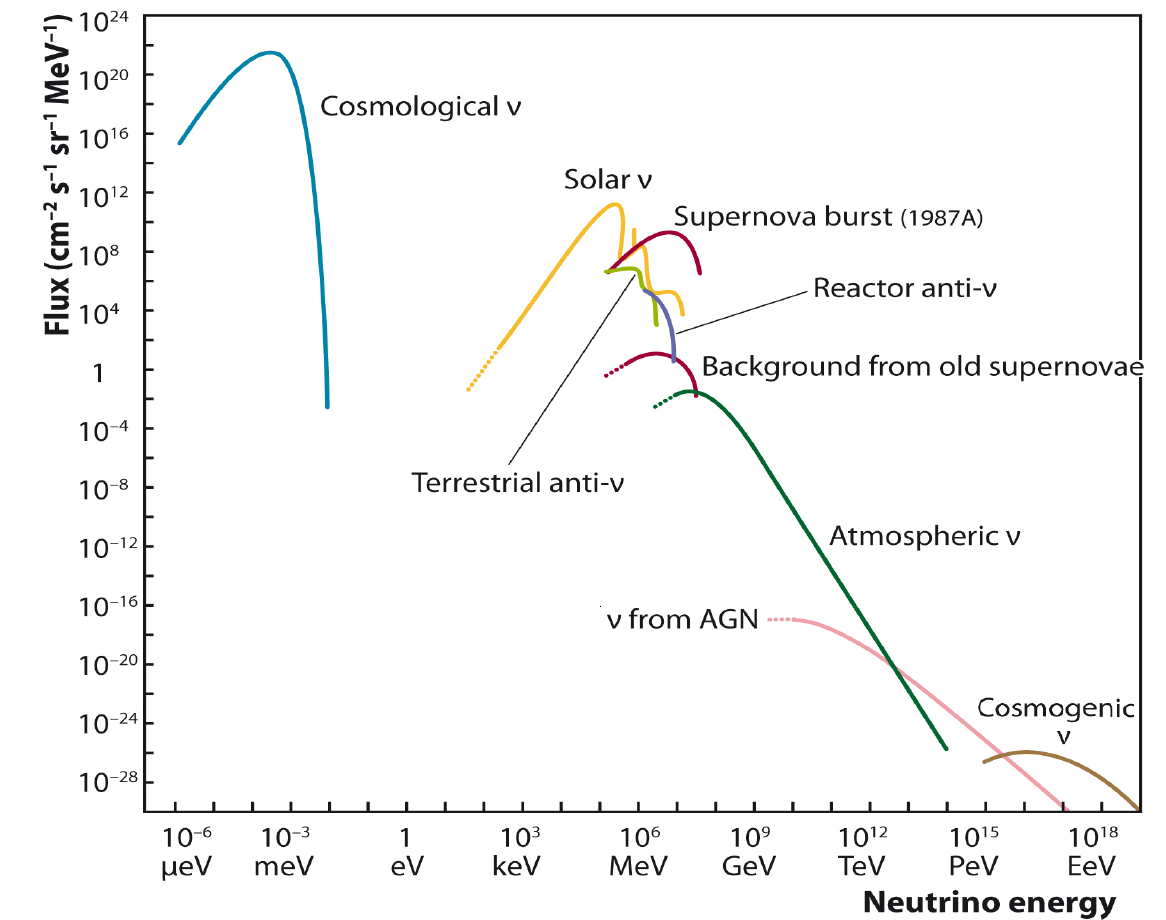
\includegraphics[width=0.75\textwidth]{content/plots/halftime/neutrinos-energy.png}
  \caption{Neutrino flux as a function of their energy.}
  \label{fig:neutrinos:flux_spectrum}
\end{figure}


% - Neutrino oscillations (not an interaction lol)
While current models of neutrino sources predict a ratio of
  $\nu_e:\nu_\mu:\nu_\tau = 1:2:0$,
the observed ratio on Earth is
  $\nu_e:\nu_\mu:\nu_\tau = 1:1:1$.
This discrepancy is explained by neutrino oscillations,
  which are a consequence of the fact that neutrinos have mass.
The mass of the neutrinos is very small,
  but it is large enough to cause oscillations between the different flavors,
  given the large distances that cosmic neutrinos travel.

\cite{neutrinos_beacom}


% - What are their interactions?
%   - Weak interaction
\subsection{Interaction with matter}
Neutrinos interact with matter via the weak interaction.
In order to compensate for the low cross-section of the weak interaction,
  the effective detector volume is maximized by utilizing existing naturally occurring detector materials,
  such as
    the Earth's atmosphere,
    the sea,
    or the ice in the Antarctic.

% - How are they detected?
%   - → IceCube, later
